\chapter{Constraining EFT parameters using Higgs boson measurements}
\label{chap:eft}

\section{Introduction}

Effective field theories were introduced in section \ref{sec:theory_eft} as a model-independent approach to constraining BSM physics. In EFT, new BSM states are assumed to exist with masses at an energy scale, $\Lambda$, far beyond the electroweak energy scale, $v$~=~246~GeV. The dynamics introduced by the BSM states can be parametrised at low energies ($E \sim v$) using higher-dimensional operators built up from the SM fields, where the operators are confined to respect both the symmetries and gauge invariance of the SM. This expansion of the SM Lagrangian, shown explicitly in equation \ref{eq:eft_expansion}, is fully general and thus can be used to constrain a wide class of BSM theories that reduce to the SM at low energies. The Wilson coefficients, $w_p$, directly parametrise the contribution from operator, $\mathcal{O}_p$, and by constraining these coefficients it is possible to infer both the strength and potential type of new BSM interactions. Ultimately, the final constraints on the Wilson coefficients can then be systematically matched to explicit UV-complete BSM theories~\cite{}.

This chapter details the application of EFT to Higgs boson property measurements at CMS. The Higgs Effective Lagrangian (HEL) is used as the language to encode modifications to Higgs boson properties from BSM physics~\cite{Contino:2013kra,Alloul:2013naa}. This interpretation is applied to the most recent CMS Higgs boson combination, documented in Ref.\cite{CMS-PAS-HIG-19-005}, which combines the measurements of cross sections in the STXS framework from multiple decay channels. In doing so, a more complete set of EFT operators, describing multiple Higgs boson interactions with other particles, can be constrained. Additionally, by performing the EFT interpretation \textit{in-house}, the fit uses the full likelihood surface, meaning no assumptions regarding the Gaussian nature of the likelihood are required.

In contrast to the $\kappa$-framework discussed in section \ref{sec:results_kappa}, the EFT approach is based on a fully consistent expansion of the SM Lagrangian. As a result, the EFT dependence can be extended from simple normalisation effects on inclusive production mode cross sections, to also capture shape variations in the kinematic distributions e.g. \ptH, \mjj, $N_{\rm{jets}}$ etc. In this interpretation, the parametrisation is defined at the granularity of the STXS framework. This ensures that the kinematic information available in STXS measurements is used to better constrain BSM physics. Additionally, the $\kappa$-framework defines coupling modifiers at LO. The EFT approach on the other hand is systematically improvable by computing higher-order contributions to the EFT predictions~\cite{Degrande:2020evl}. The interpretation shown in this chapter only considers EFT effects at LO, however the future transition to higher-orders is briefly discussed in section \ref{sec:eft_improving}.

The structure of this chapter is as follows: firstly the HEL model is described in section \ref{sec:eft_hel} and the choice of operators considered in the fit is motivated. Following this, the CMS Higgs combination~\cite{CMS-PAS-HIG-19-005} is detailed in section \ref{sec:eft_combination}, including the full set of input analyses and the extension to the statistical inference techniques introduced in chapter \ref{chap:hgg_stats}. Section \ref{sec:eft_parametrisation} discusses the EFT parametrisation of the signal yield, where the cross sections and branching ratios are expressed as functions of the Wilson coefficients, $\mu^{i,f}(\vec{w})$. These functions are then used to fit the Wilson coefficients to Higgs boson measurements, and extract their respective confidence intervals. This is performed using both a simplified re-interpretation procedure and using the full likelihood fit, described in sections \ref{sec:eft_simplified} and \ref{sec:eft_results}, respectively. Finally, the future of EFT measurements in CMS and how they can be improved is discussed in section \ref{sec:eft_improving}.

\section{Higgs Effective Lagrangian}\label{sec:eft_hel}

\textbf{This is incorrect! Re-do!}

The Higgs Effective Lagrangian (HEL) model is a partial implementation of the complete SILH basis~\cite{}, encompassing all operators at dimension-6 related to the Higgs sector. The perturbative expansion is defined in terms of a singlet scalar state, h, instead of the usual complex scalar field, H, used in the constructions of both the SM and the SMEFT~\cite{}. This choice reflects minimal assumptions in the scalar sector, and therefore can account for the possibility that the Higgs boson may deviate from the SU$_{\rm{L}}$(2) doublet nature in the SM, such as in composite Higgs models~\cite{} and theories with extra dimensions~\cite{}. The implication of this choice is that unitarity is not exactly preserved; this is not essential for EFT as long as unitarity is preserved up to the cut-off scale, $\Lambda$.

The HEL model extends the SM Lagrangian by introducing 39 flavour independent dimension-6 operators, $\mathcal{O}^{(6)}_p$, as shown in equation \ref{eq:hel_expansion}, such that new BSM dynamics in the Higgs sector would manifest itself as deviations from zero in the Wilson coefficients, $w_p$. Operators representing four-fermion interactions are not included. 

\begin{equation}\label{eq:hel_expansion}
    \mathcal{L}_{\rm{HEL}} = \mathcal{L}_{\rm{SM}} + \sum_p \frac{w_p}{\Lambda^2}\mathcal{O}^{(6)}_p .
\end{equation}

\noindent
Currently, there is insufficient data to constrain all directions of parameter space, $\vec{w}$. As a result, a subset of operators, $\{\mathcal{O}\}$  most relevant to the input Higgs boson measurements is considered. This choice ultimately introduces a model dependence into the interpretation, assuming the contribution from other operators is zero: 

\begin{equation}
  w_p=0 \; \forall \; \mathcal{O}_p \notin \{\mathcal{O}\}.   
\end{equation}

\noindent
The subset of operators considered in this analysis is motivated in section \ref{sec:eft_operator}.

The nominal HEL model is uniquely defined by the input parameters: $m_W$, $\alpha_{\rm{EM}}$ and $G_F$, where $m_W$ is the W boson mass, $\alpha_{\rm{EM}}$ is the electromagnetic coupling constant, and $G_F$ is the Fermi constant. In this input parameter scheme, the Z boson mass, $m_Z$, is dependent on the Wilson coefficients, $w_T$, $w_{WW}$, $w_B$ and $w_A$, according to equation \ref{eq:hel_mz},

\begin{equation}\label{eq:hel_mz}
    m_Z^2 = m_{Z,\rm{SM}}^2 \Big[ 1-c_T+\frac{8\,c_A\,\sin^4(\theta_W)+2\,c_{WW}\,\cos^2(\theta_W)+c_B\,\sin^2(\theta_W)}{\cos^2(\theta_W)} \Big],
\end{equation}

\noindent
where the Wilson coefficients are expressed as dimensionless quantities, $c_p$ (see section \ref{sec:eft_operator}), $m_{Z,\rm{SM}}$ is the Z boson mass in the SM, and $\theta_W$ is the Weinberg angle. In the interpretation documented here, the HEL model has been adapted to remove the $c_p$ dependence of $m_Z$, and instead fix it's value to the SM prediction. This reflects the fact that, although there is no explicit Z boson mass measurement entering the combination, it is well measured experimentally and therefore it is not physical to consider large variations in it's value. In fact, the chosen operator subset, $\{\mathcal{O}\}$, does not include $\mathcal{O}_T$, and $\mathcal{O}_{WW}$ and $\mathcal{O}_B$ are fit together in the combination of parameters, $c_{WW}-c_B$, which equation \ref{eq:hel_mz} does not explicitly depend on. The operator $\mathcal{O}_A$ is included in the subset, however the $c_A$ dependence is small ($\propto \sin^4(\theta_W)$), such that over the allowed range in $c_A$ there is a negligible shift in the $m_Z$ value, well within it's measured uncertainty. All in all, this means the treatment of $m_Z$ has a negligible effect on the measured parameters of interest. \textbf{Check this paragraph: is it theoretically sound.}

\subsection{Operator selection}\label{sec:eft_operator}
Non-zero contributions are considered in a total of eight dimension-6 operators,
\begin{equation}
    \{\mathcal{O}\} = \{\mathcal{O}_G,\mathcal{O}_A,\mathcal{O}_u,\mathcal{O}_d,\mathcal{O}_\ell,\mathcal{O}_{HW},\mathcal{O}_{WW},\mathcal{O}_B\},
\end{equation}
\noindent
where the explicit form of these operators in terms of the SM fields and the relevant Higgs boson interaction vertices are listed in Table~\ref{tab:hel_operators}. In this analysis, the nominal Wilson coefficients, $\vec{w}$, are redefined as dimensionless \textit{HEL parameters}, $\vec{c}$, which absorb the factor of $\Lambda^{-2}$. The definitions of the HEL parameters for each operator are also provided in Table~\ref{tab:hel_operators}. The operators $\mathcal{O}_G$ and $\mathcal{O}_A$ correspond to the effective Hgg and H$\gamma\gamma$ vertices, respectively. Since the interpretation presented here is a LO implementation of the HEL, the the ggH and \Hgg loops are not resolved into their SM structures and therefore only depend on $\mathcal{O}_G$ and $\mathcal{O}_A$.

This set of operators is chosen since $\vec{c}$ account for the leading CP-even terms in the scaling functions for the measured cross sections and branching ratios, and are not tightly constrained by existing measurements. CP-odd parameters are neglected as they do not enter the parametrisation at leading order in $1/\Lambda^2$, and since there is no splitting in the STXS framework that is sensitive to the Higgs boson CP (e.g. a splitting in $\Delta\phi_{jj}$) the dependence is completely degenerate with the corresponding CP-even terms at $1/\Lambda^4$.

The parameters, $c_{WW}$ and $c_B$ are fit together in the combination, $c_{WW}-c_B$, since the orthogonal combination ($S=c_{WW}+c_B$) is strongly constrained at zero by electroweak precision data~\cite{Ellis:2014jta}. Finally, the operator, $\mathcal{O}_{HB}$, is neglected. Despite having a sizeable impact on the measured quantities, the effect of $\mathcal{O}_{HB}$ is synonymous with $\mathcal{O}_{HW}$, without including additional differential measurements of the VH production mode cross sections. In conclusion, seven parameters of interest are defined:

\begin{equation}
    c_G, c_A, c_u, c_d, c_\ell, c_{HW}, c_{WW}-c_B.
\end{equation}

\begin{table}[htbp]
  \centering
  \scriptsize
  \renewcommand{\arraystretch}{2.5}
  \setlength{\tabcolsep}{3pt}
  \caption[Operator subset in the HEL interpretation]
  {
    The dimension-6 operator subset, $\{\mathcal{O}\}$, considered in the HEL interpretation. The definition of each operator is provided in terms of the SM field tensors. In addition, the corresponding HEL parameter is defined in terms of the nominal EFT Wilson coefficients. The final two columns show the affected Higgs boson interaction vertices and an example Feynman diagram of the EFT interaction. 
  }
  \label{tab:hel_operators}
%   \hspace*{-.5cm}
  \begin{tabular}{lcm{3cm}<{\centering}cm{4.5cm}<{\centering}}
    Operator & Definition & HEL Parameter & Relevant vertices & Example diagrams \\ \hline

    $\mathcal{O}_G$ & $|H|^2G^A_{\mu\nu}G^{A,\mu\nu}$ & $c_G=\frac{m_W^2}{g_s^2}\frac{w_G}{\Lambda^2}$ & Hgg & \vspace{.1cm}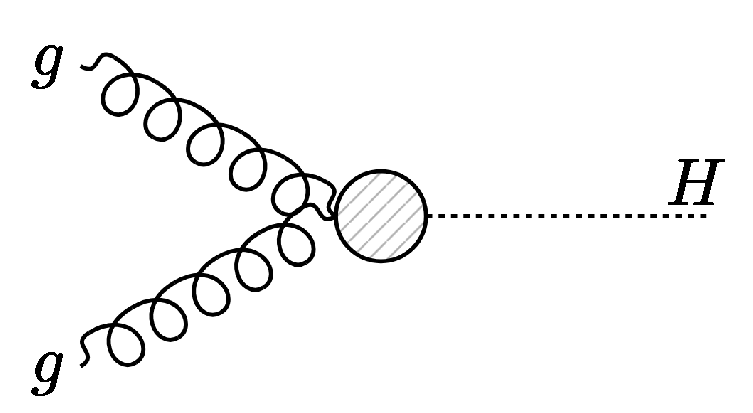
\includegraphics[width=2.5cm]{Figures/eft/eft_feynman/cG.pdf} \\

    $\mathcal{O}_A$ & $|H|^2B_{\mu\nu}B^{\mu\nu}$ & $c_A=\frac{m_W^2}{g^{'2}}\frac{w_A}{\Lambda^2}$ & H$\gamma\gamma$, HZZ & \vspace{.1cm}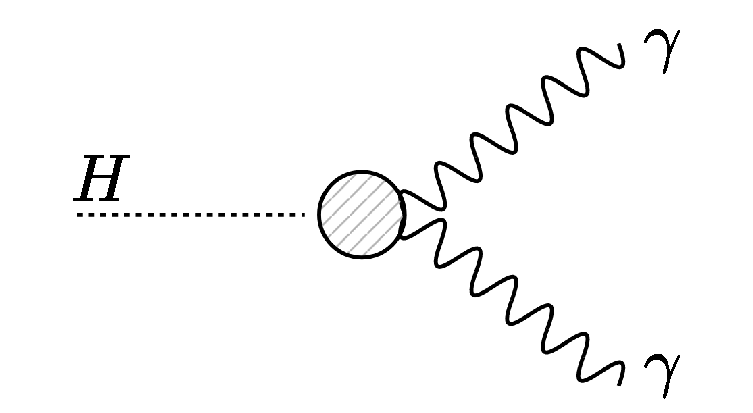
\includegraphics[width=2cm]{Figures/eft/eft_feynman/cA.pdf} \vspace{.1cm}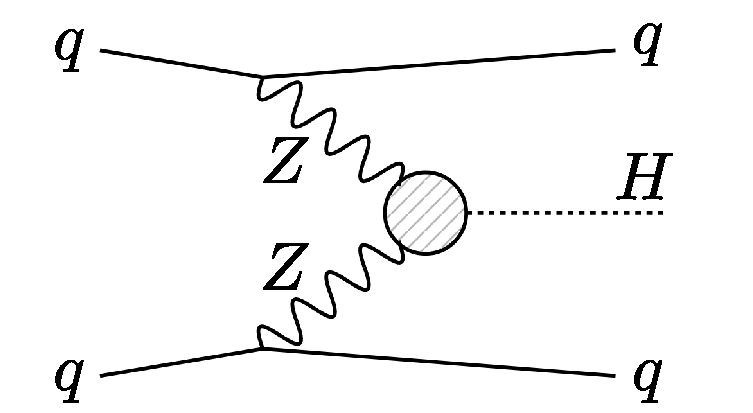
\includegraphics[width=2cm]{Figures/eft/eft_feynman/cB.pdf} \\

    $\mathcal{O}_u$ & $y_u|H|^2\bar{Q}_LH^{\dagger}u_R + {\rm{h.c.}}$ & $c_u=-v^2\frac{w_u}{\Lambda^2}$ & Htt & \vspace{.1cm}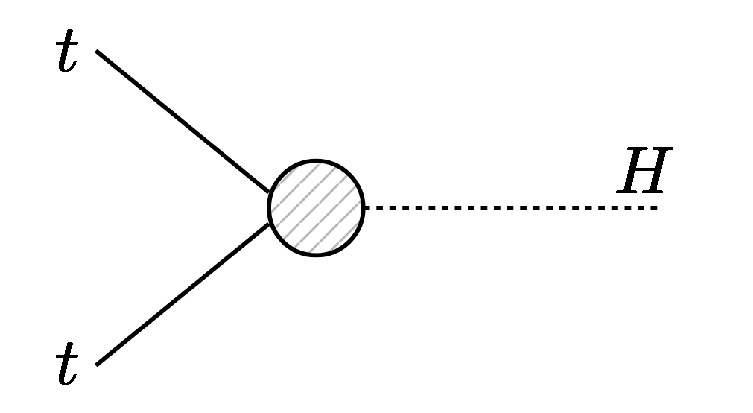
\includegraphics[width=2.5cm]{Figures/eft/eft_feynman/cu.pdf} \\

    $\mathcal{O}_d$ & $y_d|H|^2\bar{Q}_LH^{\dagger}d_R + {\rm{h.c.}}$ & $c_d=-v^2\frac{w_d}{\Lambda^2}$ & Hbb & \vspace{.1cm}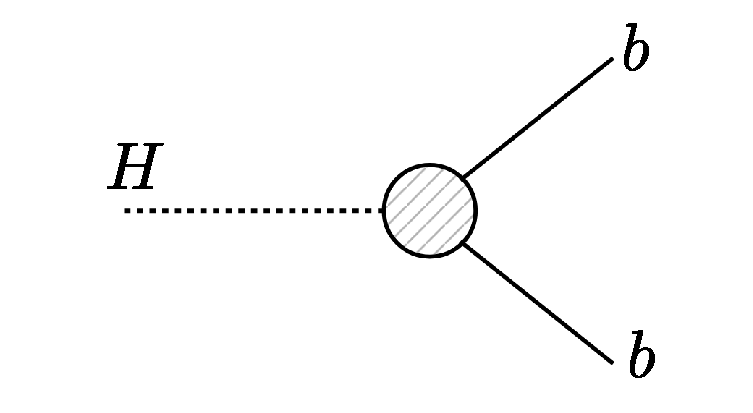
\includegraphics[width=2.5cm]{Figures/eft/eft_feynman/cd.pdf} \\

    $\mathcal{O}_\ell$ & $y_\ell|H|^2\bar{L}_LH^{\dagger}\ell_R + {\rm{h.c.}}$ & $c_\ell=-v^2\frac{w_\ell}{\Lambda^2}$ & H$\tau\tau$  & \vspace{.1cm}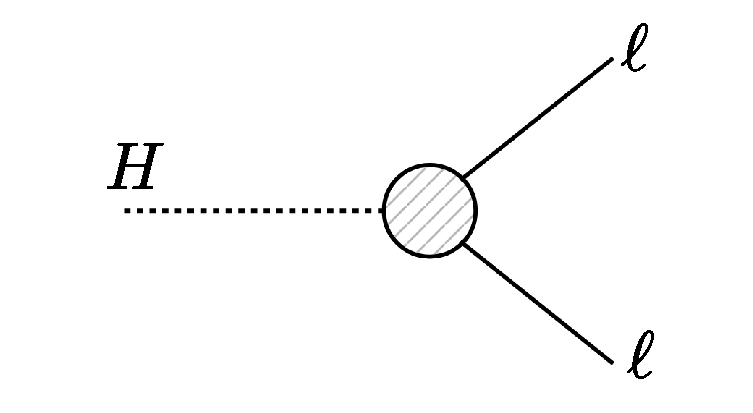
\includegraphics[width=2.5cm]{Figures/eft/eft_feynman/cl.pdf} \\

    $\mathcal{O}_{HW}$ & $i(D^\mu H)^{\dagger}\sigma^a(D^\nu H)W^a_{\mu\nu}$ & $c_{HW}=\frac{m_W^2}{2g}\frac{w_{HW}}{\Lambda^2}$ & HWW, HZZ  & \vspace{.1cm}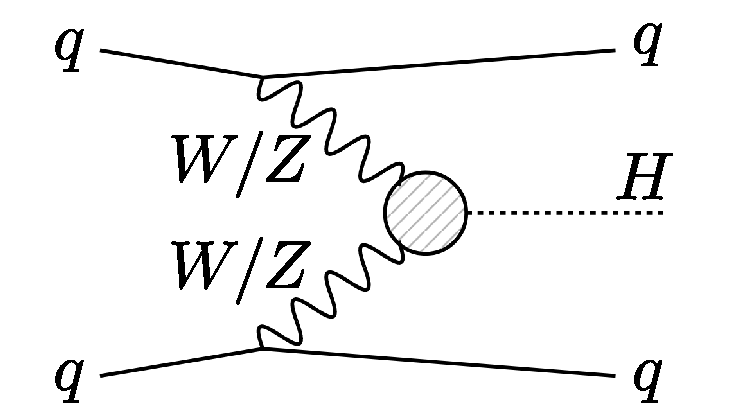
\includegraphics[width=2.5cm]{Figures/eft/eft_feynman/cHW.pdf} \\

    $\mathcal{O}_{WW}$ & $i(H^{\dagger}\sigma^aD^\mu H)D^\nu W^a_{\mu\nu}$ & $c_{WW}=\frac{m_W^2}{g}\frac{w_{WW}}{\Lambda^2}$ & HWW, HZZ & \vspace{.1cm}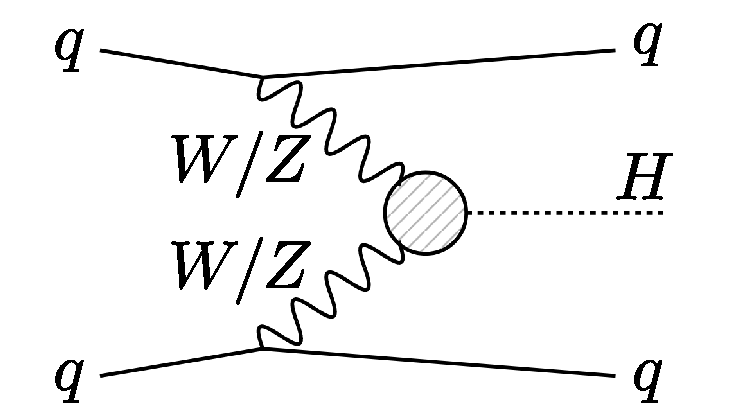
\includegraphics[width=2.5cm]{Figures/eft/eft_feynman/cHW.pdf} \\

    $\mathcal{O}_B$ & $i(H^{\dagger}D^\mu H)\partial^\nu B_{\mu\nu}$ & $c_{WW}=\frac{2m_W^2}{g'}\frac{w_{B}}{\Lambda^2}$ & HZZ & \vspace{.1cm}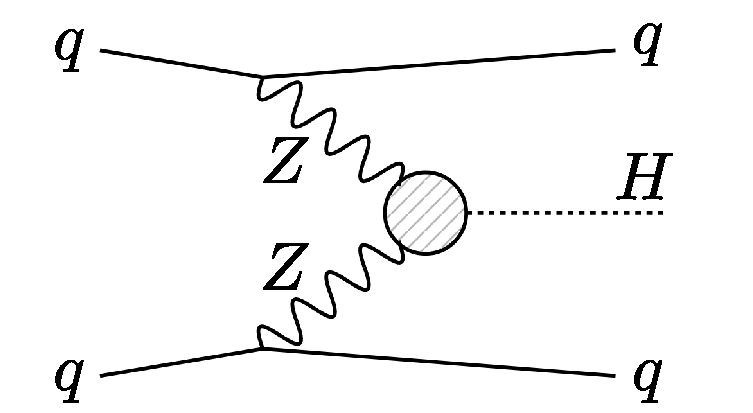
\includegraphics[width=2.5cm]{Figures/eft/eft_feynman/cB.pdf} \\

\end{tabular}
%   \hspace*{-.5cm}
\end{table}

\section{CMS Higgs combination}\label{sec:eft_combination}
The HEL interpretation is applied to the latest Higgs boson combination performed by the CMS experiment, documented in Ref.~\cite{CMS-PAS-HIG-19-005}. The combination includes analyses targeting all the major Higgs boson decay channels, with integrated luminosities ranging from 35.9~\fbinv to 137~\fbinv, depending on the input analysis. By targeting different final states, most analyses are orthogonal by construction. For similar final states, the overlap in the selected events has been checked and found to be negligible. 

The inclusion of different decay channels ensures sensitivity to a larger subset of operators (see Table~\ref{tab:hel_operators}). Each input analysis measures cross sections in the STXS framework; however, these measurements are performed at different \textit{stages} which define binning schemes of varying granularity.
As a result, the EFT parametrisation of the signal yield is defined at the granularity of all STXS stages which enter the combination: stage 0, 1.0 and 1.1. For stage 1.0 and above, the bins are split according to the event kinematics (e.g. \ptH, $N_{\rm{jets}}$ etc), and as a result the kinematic information available in these measurements is used to further constrain BSM effects beyond simple inclusive effects.

The full list of input analyses is provided in Table~\ref{tab:combination_inputs}. Note, this combination was performed before the \Hgg analysis described in chapters~\ref{chap:hgg_overview}--\ref{chap:hgg_results}, and so the \Hgg inputs are taken from previous analyses. For each decay channel, the targeted production modes and final states are listed, in addition to the STXS stage of the measurements and the integrated luminosity of the data set used in the corresponding analyses. More detailed information on each input analysis can be found in the corresponding references.

\textbf{Add input analysis table here}.

\subsection{Statistical procedure}
The statistical inference procedure used in the combination is a simple extension to that described in sections \ref{sec:category_likelihood} and \ref{sec:results_extraction}. A likelihood function\footnote{The dependence of the likelihood on the Higgs boson mass, $m_H$, has been dropped from the notation. For the form of the Poisson terms, please refer to equation \ref{eq:poisson_def}.} is constructed for each analysis category or \textit{region}, $k$, now defined for a generic final state, $f$,

\begin{equation}
    L_k({\rm{data}}\,|\,\vec{\alpha},\vec{\theta}_s,\vec{\theta_b}) = \mathcal{P}_k( {\rm{data}}\,|\,\vec{\alpha},\vec{\theta_s},\vec{\theta}_b),
\end{equation}

\noindent
where the quanta of the likelihood, $\mathcal{P}_k$, takes the following form for binned analysis regions,

\begin{equation}
    \mathcal{P}^{\rm{binned}}_k = \prod^{N_{\rm{bins}}}_X {\rm{Poisson}}\Big( N^{\rm{data}}_{k,X} \, \Big| \, \Big[\sum_{i,f} S^{i,f}_{k,X}(\vec{\alpha},\vec{\theta}_s) \Big] + B_{k,X}(\vec{\theta}_b) \Big).  
\end{equation}
\noindent
Here, the index $X$ runs over bins of some observable(s) e.g. \mgg for the \Hgg analyses. The quantity $S^{i,f}_{k,X}$ corresponds to the signal estimate in bin $X$, of analysis region $k$, originating from STXS bin, $i$, and decaying to final state, $f$. The background estimate and number of data events in the same observable bin are referred to as $B_{k,X}$ and $N^{\rm{data}}_{k,X}$, respectively. For unbinned analysis regions, the quanta is defined as,

\begin{equation}
    \mathcal{P}^{\rm{unbinned}}_k = \frac{1}{z} \prod^{z}_j {\rm{Poisson}}\Big(1 \, \Big| \, \Big[\sum_{i,f} S^{i,f}_{k}(\vec{\alpha},\vec{\theta}_s) \cdot \rho^{i,f}_{k,{\rm{sig}}}(x_j|\vec{\alpha},\vec{\theta}_s) \Big] + B_{k}(\vec{\theta}_b)\cdot \rho_{k,{\rm{bkg}}}(x_j|\vec{\theta}_b) \Big),
\end{equation}

\noindent
for $z$ events in data landing in region $k$, where each event is labelled by the index $j$. The terms $\rho^{i,f}_{k,{\rm{sig}}}(x)$ and $\rho_{k,{\rm{bkg}}}(x)$ are the probability density functions of some observable(s) $x$, for signal and background, respectively. The total signal and background yield estimates in region $k$ are expressed by $S^{i,f}_{k}$ and $B_{k}$. Comparing to the binned scenario, $S^{i,f}_{k}$ and $B_{k}$, are equal to the sum of the $S^{i,f}_{k,X}$ and $B_{k,X}$ terms over all observable bins, $X$. In all equations, it is assumed that the background estimate does not depend on the parameters of interest, $\vec{\alpha}$, which may not always be the case in a fully consistent EFT framework (see section \ref{sec:eft_improving}). Also, the modelling of the signal in terms of the observable(s) is extracted using the SM template, and is assumed to be independent of $\vec{\alpha}$: $\rho^{i,f}_{k,{\rm{sig}}}(x|\vec{\alpha},\vec{\theta})=\rho^{i,f}_{k,{\rm{sig}}}(x|\vec{\theta})$. For example, the shape of the signal \mgg peak in the \Hgg analysis is not parametrised as a function of the HEL parameters.

In the EFT interpretation, the signal yield for STXS bin, $i$, in final state, $f$, landing in analysis region, $k$ is expressed as, 

\begin{equation}\label{eq:signal_yield_eft}
    S_k^{i,f} = \mu^{i,f}(\vec{c}) \times \big[\sigma^i \cdot \mathcal{B}^{f} \big]_{\rm{SM}} \times \epsilon^{i,f}_k(\vec{c}) \times \mathcal{L}.
\end{equation}

\noindent
This is effectively an extension of equation \ref{eq:signal_yield}, where the explicit dependence on the HEL parameters, $\vec{c}\,(\equiv\vec{\alpha})$ is stated. Note, the dependence on the nuisance parameters, $\vec{\theta}$, has been dropped from the notation for simplicity. The extraction of the cross section times branching ratio scaling functions, $\mu^{i,f}(\vec{c})$, is described in section~\ref{sec:eft_parametrisation}. Interestingly, since the EFT operators can distort the event kinematics away from the SM hypothesis, the efficiency times acceptance values, $\epsilon^{i,f}_k(\vec{c})$ become dependent on the HEL parameters. This is especially true for measurements in the STXS framework, where the products of the Higgs boson decay are not restricted to fiducial phase space definitions. Nevertheless, in this interpretation, the so-called \textit{acceptance corrections} are ignored: $\epsilon^{i,f}_k(\vec{c})=\epsilon^{i,f}_k$. The potential impact of fully accounting for the detector efficiencies and analysis acceptance is investigated in section \ref{sec:eft_acceptance_corrections}.

The total likelihood is now defined as the product of the analysis region likelihood functions, taken over all input analyses included in the combination,

\begin{equation}
    L({\rm{data}}\,|\,\vec{\alpha},\vec{\theta}) = \prod_{k}^{N_{\rm{regions}}} \Big[    L_k({\rm{data}}\,|\,\vec{\alpha},\vec{\theta}) \,\Big] \times \mathcal{C}(\vec{\theta}) ,
\end{equation}

\noindent
where the constraint term, $\mathcal{C}$, takes the same form of that shown in section \ref{sec:category_likelihood}, such that deviations from the expected values of the nuisance parameters are penalised according to the associated prior. Since the different input analyses can have common sources of systematic uncertainty, the corresponding nuisance parameters must be correlated across decay channels. This follows the same procedure as described in section \ref{sec:correlation_scheme}, where in addition to defining per-year correlations, a single nuisance parameter is defined in the construction of the likelihood which affects the yield estimate in multiple decay channels simultaneously. 

All theoretical uncertainties arising from the renormalisation and factorisation scales used in the cross section calculations\footnote{This includes both the inclusive effects and the uncertainties modelling migrations \textit{across} STXS bins}, the parton distribution functions, and the branching ratio predictions are treated as fully correlated across decay channels. In addition, since other analyses use MC to estimate background contributions, it is necessary in these cases to introduce the uncertainties in the theoretical predictions of the background cross sections. These uncertainties are correlated between channels in which the same background appears. The results presented in this section are an \textit{interpretation} of cross section measurements, therefore the theory uncertainties directly affecting $[\sigma^i \cdot \mathcal{B}^{f}]_{\rm{SM}}$ are folded into the measurement.

Most experimental uncertainties are analysis specific (e.g. \mgg signal shape uncertainties), and are therefore uncorrelated. However, there are a number of exceptions. This includes the uncertainties in the luminosity estimates, the lepton efficiency scale factors, the jet energy scale and resolution, and the b tagging efficiency. For most channels, which do not use a specific treatment of the aforementioned uncertainty sources, they are treated as correlated nuisance parameters. More information regarding the experimental uncertainty correlation scheme is provided in Ref.~\cite{CMS-PAS-HIG-19-005}.

After the total likelihood function has been constructed, the method of extracting the final results is identical to that described in section \ref{sec:results_extraction}.

\subsection{Results in the signal strength parametrisation}
Figure \ref{fig:combination_mu} shows the results of the CMS Higgs boson combination in the signal strength parametrisation. An independent signal strength modifier, $\mu_i^f$, has been introduced to scale each production mode, $i$, times decay channel, $f$. The observed correlations between the fitted signal strengths are displayed in Figure \ref{fig:combination_mu_corr}.

\begin{figure}[htbp]
  \centering
  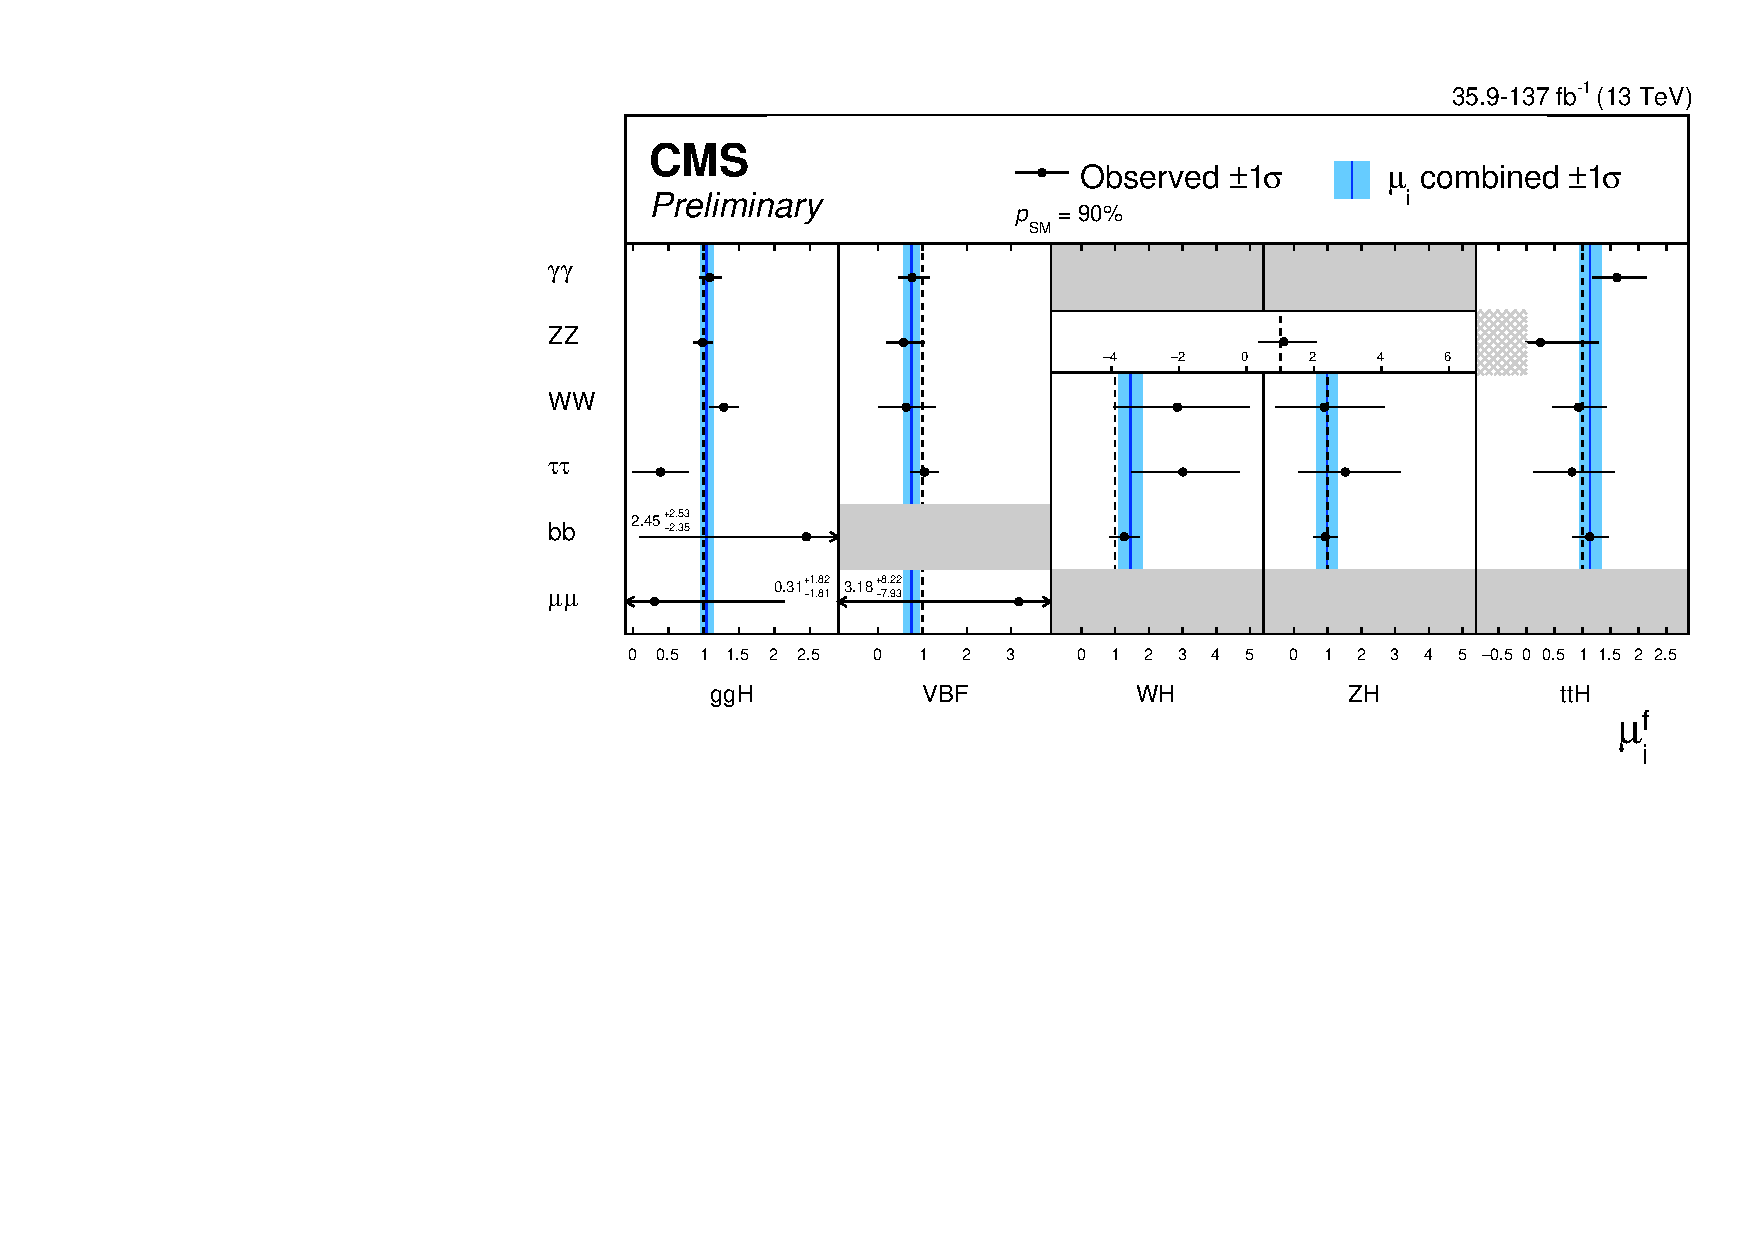
\includegraphics[width=.8\textwidth]{Figures/eft/combination_mu.pdf}
  \caption[Results of the combination signal strength fit]
  {
    Observed best-fit values (black points) and 68\% confidence intervals (black lines) for the signal strength modifiers, $\mu_i^f$. The grey filled boxes indicate signal strength modifiers which are not included in the fit, since there is no input measurement targeting them. The hatched grey box indicates the restricted region in $\mu^{ZZ}_{ttH}$ for which the total signal plus background probability density function goes negative. For \HZZ, the WH and ZH production modes are fit together using a common signal strength modifier. This fit is extrememly compatible with the SM, with a corresponding $p$-value of approximately $p_{\rm{SM}}=90\%$. The blue bands indicate the results of a different parametrisation which introduces a per-production mode signal strength modifier, combined across decay channels. 
  }
  \label{fig:combination_mu}
\end{figure}

\begin{figure}[htbp]
  \centering
  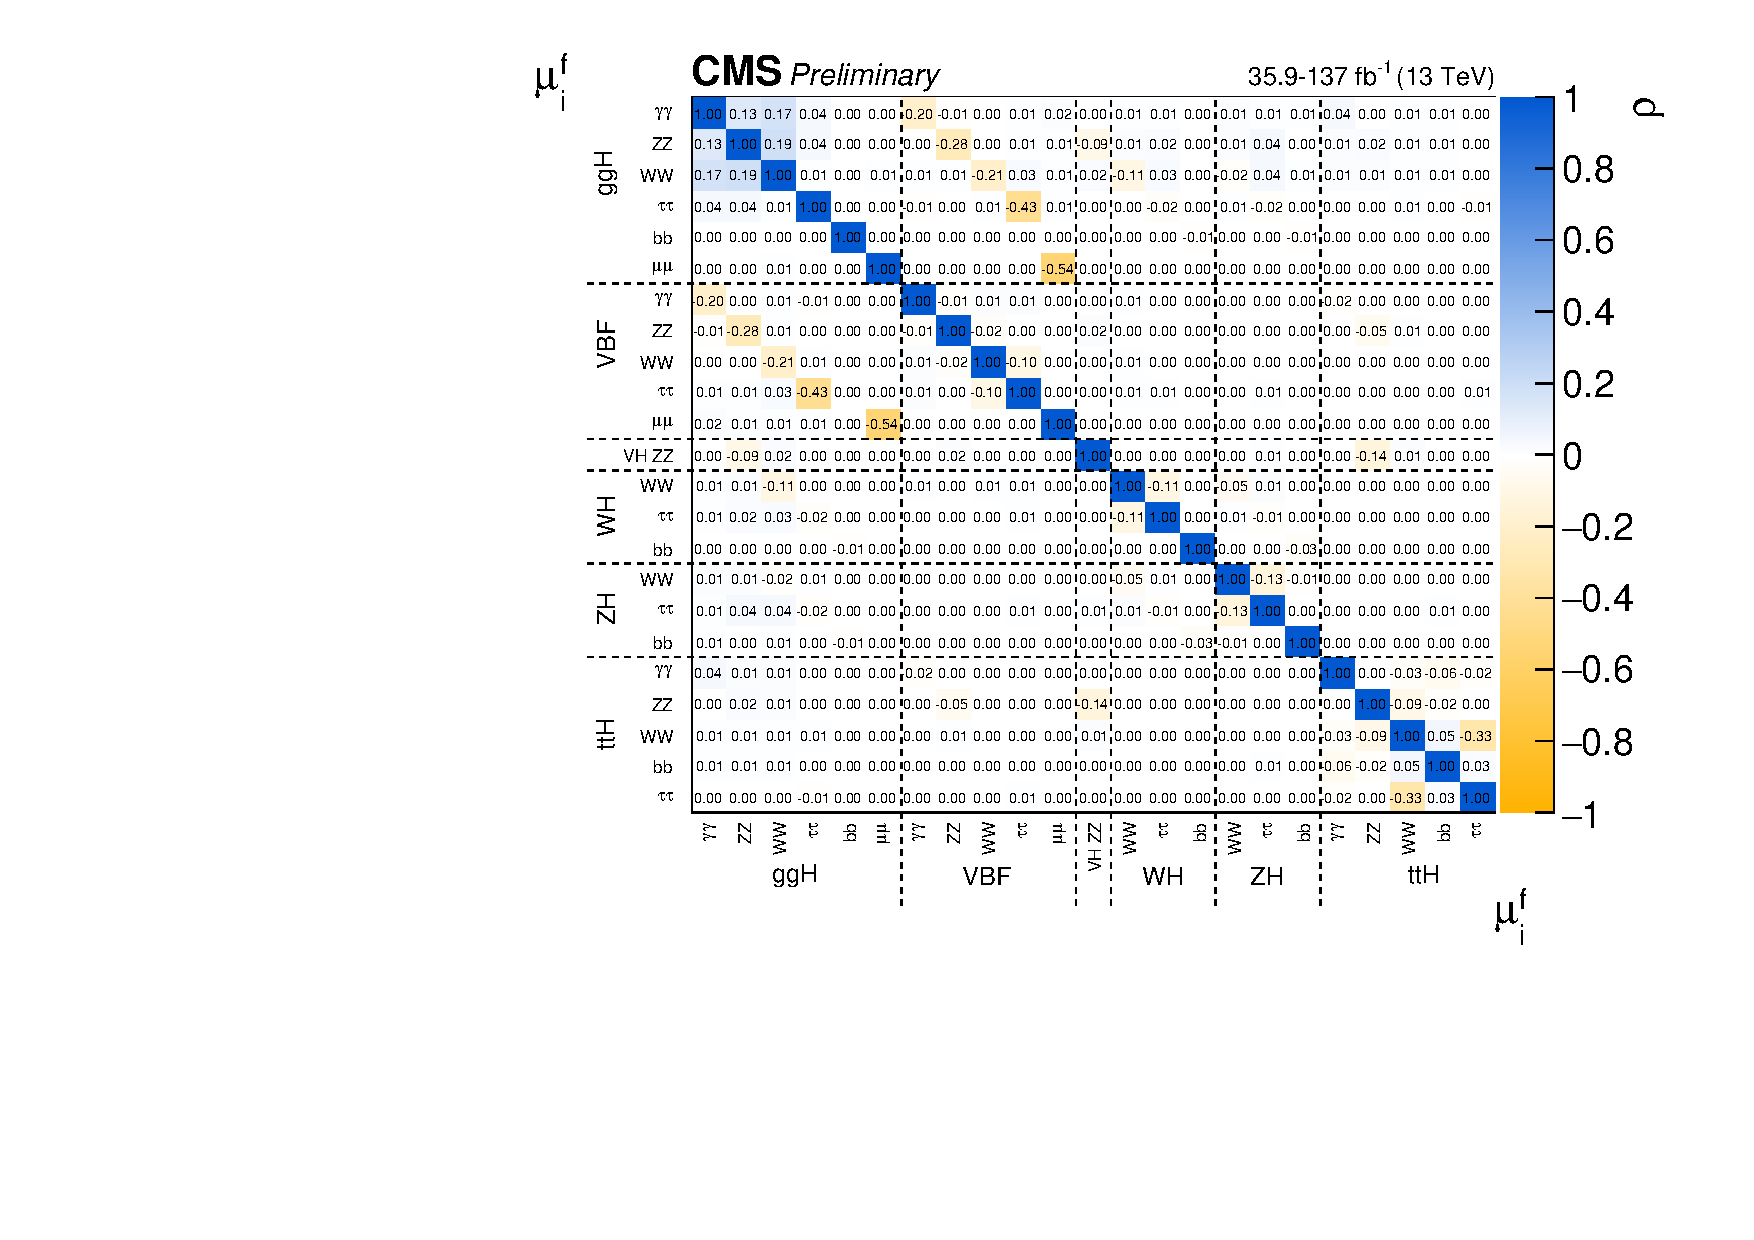
\includegraphics[width=.75\textwidth]{Figures/eft/combination_mu_corr.pdf}
  \caption[Correlations in the combination signal strength fit]
  {
    Observed correlations between the fitted signal strengths. The size of the correlations is indicated by the colour scale.
  }
  \label{fig:combination_mu_corr}
\end{figure}

\newpage
\section{Signal yield parametrization}\label{sec:eft_parametrisation}
The scaling functions, $\mu^{i,f}(\vec{c})$, shown in equation \ref{eq:signal_yield_eft}, parametrise the signal cross section times branching ratios as a function of HEL parameters, and are derived as follows. Within the HEL framework (equation \ref{eq:hel_expansion}) the amplitude for each Higgs boson production and decay process can be described as,

\begin{equation}\label{eq:hel_matrixelement}
    |\mathcal{M}_{\rm{HEL}}|^2 = \Big| \mathcal{M}_{\rm{SM}} + \mathcal{M}_{\rm{BSM}} \Big|^2 = |\mathcal{M}_{\rm{SM}}|^2 + 2{\rm{Re}}\{\mathcal{M}_{SM}\mathcal{M}^{\dagger}_{\rm{BSM}}\} + |\mathcal{M}_{\rm{BSM}}|^2,
\end{equation}

\noindent
where $\mathcal{M}_{\rm{SM}}$ and $\mathcal{M}_{\rm{BSM}}$ are the matrix elements originating from the SM and BSM parts of the Lagrangian, respectively. The total amplitude now contains an SM-BSM interference term, suppressed by a factor of $\Lambda^{-2}$, and a purely-BSM term, suppressed by a factor $\Lambda^{-4}$. In this interpretation, only one BSM vertex is considered per Feynman diagram, which means $\mathcal{M}_{\rm{BSM}}$ is linear in the HEL Wilson coefficients. Substituting this linearity condition into equation \ref{eq:hel_matrixelement}, and using the fact $\sigma \propto |\mathcal{M}|^2$, we arrive at an expression for the cross section of signal process, $i$,

\begin{equation}
    \sigma^i_{\rm{HEL}} = \sigma^i_{\rm{SM}} + \sigma^i_{\rm{int}} + \sigma^i_{\rm{BSM}},
\end{equation}

\noindent
which results in a scaling function quadratic in the HEL parameters,

\begin{equation}
    \mu^i_{\rm{prod}}(\vec{c}) = \frac{\sigma^i_{\rm{HEL}}}{\sigma^i_{\rm{SM}}} = 1 + \sum_p A^i_p\,c_p + \sum_p \sum_r B^i_{pr}\,c_p\,c_r,
\end{equation}

\noindent
where in this analysis, $i$, corresponds to the STXS bin. The terms, $A^i_p$ and $B^i_{pr}$, are constant prefactors which encode the impact of the HEL parameters on each bin. The $|\mathcal{M}_{\rm{BSM}}|^2$ can be dropped by neglecting the $B^i_{pr}$ prefactors. Despite having an energy scale suppression of the same order as the leading dimension-8 SM-BSM interference contributions ($\Lambda^{-4}$), the $B^i_{pr}$ terms are kept here since they are the leading purely-BSM terms and they prevent the scaling functions from going negative, thus leading to a better fit to data.

Applying the same reasoning, the partial Higgs boson decay width to final state $f$ scales relative to the SM prediction as,

\begin{equation}
    \frac{\Gamma^f_{\rm{HEL}}}{\Gamma^f_{\rm{SM}}} = 1 + \sum_p A^f_p\,c_p + \sum_p \sum_r B^f_{pr}\,c_p\,c_r.
\end{equation}

\noindent
It is necessary to also consider the variation in the total Higgs boson decay width, $\Gamma^H$, such that the scaling function of the branching ratio to final state f is expressed as,

\begin{equation}
    \mu^f_{\rm{decay}}(\vec{c}) = \frac{\mathcal{B}^f_{\rm{HEL}}}{\mathcal{B}^f_{\rm{SM}}} = \frac{\Gamma^f_{\rm{HEL}}/\Gamma^f_{\rm{SM}}}{\Gamma^H_{\rm{HEL}}/\Gamma^H_{\rm{SM}}} = \frac{1 + \sum\limits_p A^f_p\,c_p + \sum\limits_p \sum\limits_r B^f_{pr}\,c_p\,c_r}{1 + \sum\limits^{~}_p A^H_p\,c_p + \sum\limits_p \sum\limits_r B^H_{pr}\,c_p\,c_r}.
\end{equation}

The total scaling function for signal events originating from STXS bin, $i$, and decaying to final state, $f$, is the product of the individual cross section and branching ratio scaling functions,

\begin{equation}
    \mu^{i,f}(\vec{c}) = \mu^i_{\rm{prod}}(\vec{c}) \cdot \mu^f_{\rm{decay}}(\vec{c}).
\end{equation}

\noindent
This works under the narrow Higgs boson width assumption, such that the effects at production and decay have been factorised. These scaling functions are uniquely described by the set of constant prefactors: $\{A^i_p,B^i_{pr},A^f_p,B^f_{pr},A^{H}_p,B^{H}_{pr}\}$, which are derived using LO MC samples with the reweighting procedure described in section \ref{sec:hel_derivation}. It should be stressed that the SM predictions for the cross sections and branching ratio in equation \ref{eq:signal_yield_eft} are computed at the highest available order, however the EFT parametrisation is derived using LO MC samples. This strategy therefore assumes that the corrections to the cross sections and branching ratios from HEL operators is comparable at LO and higher orders~\cite{Degrande:2016dqg}. Once defined, the scaling functions are then applied in the likelihood fit to extract the best-fit values and corresponding confidence intervals for the considered HEL parameters. 


\subsection{Derivation: Monte Carlo reweighting}\label{sec:hel_derivation}
The impact of the HEL operators is computed using the \texttt{HEL\_UFO} model~\cite{Alloul:2013naa} in Madgraph~\cite{Alwall:2014hca}, where the Higgs boson production and decay processes are generated at LO in both QCD and QED. The LO Madgraph reweighting functionality~\cite{Mattelaer:2016gcx} is utilised, to reweight the generated events to different points in the HEL parameter space, according to,

\begin{equation}
    W_{\vec{c}} = \frac{|\mathcal{M}^{\vec{c}}_{\rm{HEL}}|^2}{|\mathcal{M}^{\rm{nominal}}_{\rm{HEL}}|^2} \cdot W_{\rm{nominal}}
\end{equation}

\noindent
where $\mathcal{M}^{\vec{c}}_{\rm{HEL}}$ is the matrix element at the point in parameter space, $\vec{c}$, $\mathcal{M}^{\rm{nominal}}_{\rm{HEL}}$ is the matrix element at the nominal point, and $W_{\rm{nominal}}$ is the corresponding event weight at that nominal point. Here, the nominal point in parameter space is chosen as the SM: $\vec{c} = (0,0,...,0)$.

For each operator, $\mathcal{O}_p$, two weights are defined by setting $c_p$ to two different values ($a$,$2a$), whilst all other HEL parameters are kept at 0. In doing so, two simultaneous equations are constructed, as shown in \ref{eq:HEL_simultaneous}, where the reweighted and SM values of the observable, $X$ ($\sigma^i$ for production, $\Gamma^f$ for decay), can be used to infer the values of $A_p$ and $B_{pp}$,

\begin{equation}\label{eq:HEL_simultaneous}
    \begin{split}
        \frac{X_{c_p=a}}{X_{\rm{nominal}}} = 1 + a \cdot A_p + a^2 \cdot B_{pp} \\
        \frac{X_{c_p=2a}}{X_{\rm{nominal}}} = 1 + 2a \cdot A_p + 4a^2 \cdot B_{pp}.
    \end{split}
\end{equation}

\noindent
An additional weight is required to extract the cross-terms, $B_{pr}$ where $p \neq r$. This is defined by setting $(c_p,c_r)=(a,a)$, and keeping all other HEL parameters at 0, such that,

\begin{equation}
    \frac{X_{(c_p,c_r)=(a,a)}}{X_{\rm{nominal}}} = 1 + a \cdot (A_p+A_r) + a^2 \cdot (B_{pp}+B_{rr}+B_{pr}).
\end{equation}

\noindent
The value of $B_{pr}$ can then be inferred by using the previously calculated prefactors, $\{A_p,A_r,B_{pp},B_{rr}\}$, from equation \ref{eq:HEL_simultaneous}. In total, the number of weights required to fully specify the scaling functions is,

\begin{equation}
    N_{\rm{weights}} = 1 + 2N + \frac{N(N-1)}{2},
\end{equation}

\noindent
where $N$ is the number of operators; this analysis considers 8 HEL operators and therefore requires 45 weights, including the nominal SM weight. The value of $a$ is chosen to be small (0.001 CHECK!) to ensure the EFT effects do not blow up in the matrix element calculations, and therefore do not invoke a large statistical uncertainty in the calculated prefactors.

No additional generator-level kinematic cuts are applied except the default ones in Madgraph. All events are interfaced with \textsc{Pythia8} for parton showering and hadronisation~\cite{}. A matching is performed to remove phase space overlap between jets specified in the matrix element and those originating from the parton shower. The XXX algorithm is used for all processes, with a matching parameter of XX~GeV~\cite{}. 

Many of the option choices used in the event generation can affect the values of the prefactors, and therefore the scaling functions. For example, the EFT effects originate solely from the matrix element (in Madgraph) and not from the parton showering (in \textsc{Pythia8}). Therefore, the values of the prefactors can depend on the scheme and parameters used for the jet matching. In general, these generator options have a small effect on the final parametrisation, nevertheless it is important to specify the options used when reporting results. A summary of the MC options used in this analysis is provided in Appendix~\ref{app:generator_options}.

\subsection{Effect at production}
Each Higgs boson production mode is generated separately, according to the Madgraph process definitions listed in Appendix~\ref{app:generator_options}. The Higgs boson decay is not specified in the process definition, such that EFT effects only enter in the Higgs boson production interaction vertices. The option \texttt{NP<=1} limits the events to one BSM vertex per diagram. After interfacing with \textsc{Pythia8}, the particle-level events are propagated through the Rivet program~\cite{}, using the \texttt{HiggsTemplateCrossSections} routine~\cite{}. This routine sequentially extracts the simulated event constituents, forms hadronic jets using the anti-$k_T$ algorithm with a distance parameter of 0.4~\cite{}, calculates high-level kinematic quantities (e.g. \ptH, \ptV, \ptHjj, \mjj, $N_{\rm{jets}}$) and, finally, \textit{classifies} the simulated events according to their truth-level STXS bin. In all steps including the classification, the Higgs boson decay products formed by \textsc{Pythia8} are neglected. The routine has been modified to output the bin classification at each stage of the STXS framework considered in the combination: stage 0, 1.0 and 1.1.

A large number of events are generated for each production mode ($10^6$) to ensure each STXS bin is sufficiently populated. As a result the uncertainty in the scaling function prefactors arising from the limited MC statistics is small (typically below 1\%). The set of 45 event weights are then applied to extract the SM and EFT reweighted cross sections of each individual STXS bin, which are subsequently used to calculate the relevant prefactors: $\{A^i_p,B^i_{pr}\}$, according to the prescription described above. 

Figure \ref{fig:zhlep_ptv} shows the \ptV distribution for ZH lep events in the SM (black line) and when turning on various HEL parameters (coloured lines). The enhancement due to the XX and YY parameters grows with increasing \ptV; measuring this region of phase space well would allow for tighter constraints on these parameters. The dashed lines in the plot indicate the boundaries in \ptV which define the ZH lep STXS stage 1.1 bins. In addition, the ZH lep $150<\ptV<250$~GeV region is further split into bins with zero jets and at least one jet. The cross section scaling functions, $\mu^i(\vec{c})$, for each of these bins are shown as a function of the relevant HEL parameters in Figure \ref{fig:zhlep_sf_1d}. In the plots, all other HEL parameters apart from the dependent variable are set to zero. Going further, Figure \ref{fig:zhlep_sf_2d}, shows $\mu^i(\vec{c})$ for the ZH lep $\ptV>250$~GeV STXS bin, considering variations in pairs of HEL parameters: $c_{WW}$-vs-$c_B$ and $c_{WW}$-vs-$c_{HW}$. The tilt in the distributions arises from the relevant cross-terms, $B_{pr}$ for $p \neq r$.

\begin{itemize}
    \item 1D scaling functions for ZH lep. Include uncertainty?
    \item 2D scaling function for single STXS bin of ZH lep
\end{itemize}

The scaling functions for the inclusive ttH STXS bin (ttH is only split at stage 1.2) is shown as a function of $c_u$ (left) and $c_G$ (right) in Figure \ref{fig:tth_sf_1d}. Interestingly, the scaling function is equal to unity for two distinct values of $c_u$ within the allowed range of the parameter: at the SM point ($c_u=0$) and at $c_u=-4/3$. Without additional measurements sensitive to $c_u$ entering the likelihood, it is impossible to distinguish between these two points in parameter space. As a result the $q(c_u)$ curve will exhibit a double minimum structure, with minima situated around $c_u=0$ and $c_u=-4/3$. The inclusion of the tH production cross section measurement shown in chapter \ref{chap:hgg_results} would help alleviate this degeneracy.

\begin{itemize}
    \item 1D scaling functions for ttH
\end{itemize}


\subsection{Effect at decay}
The decay mode parametrisation is taken directly from Ref.~\cite{Hays:2673969}. Higgs bosons are generated at rest and are made to decay in a particular channel in the matrix element definition (see Appendix~\ref{app:generator_options}), such that EFT effects enter the Higgs boson decay vertices. The STXS framework does not include a fiducial region definition for the Higgs boson decay products, and therefore the EFT effects at decay are independent of the Higgs boson kinematics. If the acceptance effects were considered ($\epsilon^{i,f}_k(\vec{c})$), it would be necessary to generate the Higgs boson with a non-zero momentum spectrum to correctly describe the phase space of the decay products. 

The partial width scaling functions are derived using a similar approach to the cross section scaling functions. This amounts to extracting the SM prediction of the partial width at LO and the partial width with EFT effects turned on, and following the derivation procedure outlined in section \ref{sec:hel_derivation}. The total Higgs boson decay width parametrisation is then inferred from the sum of all partial width scalings, where the decay channels are weighted in the sum according to their total contribution to $\Gamma^{H}$. Figure \ref{fig:eft_decay} summarises the branching ratio scaling functions, $\mu_{\rm{decay}}^f(\vec{c})$, for the decay channels considered in the CMS Higgs boson combination. Similar to ttH production, the \Hbb and \Htautau scaling functions have two points in $c_d$ and $c_\ell$ respectively, which correspond to the SM prediction (unity). Again, since no additional measurements are included in the combination which are sensitive to these parameters, the corresponding $q(c_d)$ and $q(c_\ell)$ curves will exhibit a double-minimum structure.

\begin{itemize}
    \item Branching ratio scaling functions: split into partial width and total width contributions. One plot for each HEL parameter.
\end{itemize}

\subsection{Summary}
The impact of each HEL parameter on the stage 0, 1.0 and 1.1 cross sections, and the branching ratios is displayed in Figure \ref{fig:hel_summary}, relative to the SM predictions. Each parameter is varied to it's expected upper 68\% confidence level value to indicate the size of variations to which the combined measurements are sensitive to. For parameters which demonstrate a double-minimum in the likelihood ($c_u$,$c_d$,$c_\ell$), the upper confidence level is taken from the minimum around 0. 

\begin{itemize}
    \item Big summary plot: similar to ATLAS one
\end{itemize}

The full HEL parametrisation, $\mu_{\rm{prod}}^i(\vec{c})$ and $\mu_{\rm{decay}}^f(\vec{c})$, is presented in Tables XX-YY of Appendix~\ref{app:hel_parametrisation}. The total scaling function is defined as the product of the corresponding cross section and branching ratio scaling functions. Figure \ref{fig:hel_total_gghhgg} shows the example for ggH in the \Hgg decay channel, plotted as a function of $c_G$-vs-$c_A$. These total scaling functions are applied to the signal yield estimates when constructing the likelihood, as shown in equation \ref{eq:signal_yield_eft}, and constraints on the HEL parameters, $\vec{c}$, are extracted using the techniques described in section \ref{sec:results_extraction}.

\begin{itemize}
    \item Total scaling: ggH \Hgg
\end{itemize}

\subsection{Validation of the scaling functions}
The cross section scaling functions have been calculated previously for the stage 1.0 bin definitions in Ref.~\cite{Hays:2673969}. This enables a direct comparison with the prefactors, $A_p$ and $B_{pr}$, calculated here. 
Something about the 20\% improvement in the constraints.

\section{Simplified likelihood re-interpretation procedure}\label{sec:eft_simplified}
This section serves as an aside to the rest of this chapter and can be skipped without loss of understanding. Nevertheless, before showing the results extracted using the full likelihood, it is useful to introduce a simplified approach to re-interpreting cross section measurements. This has been used as a tool to investigate particular properties of the HEL interpretation, such as the most important operators for the combination input analyses, and to gain an estimate of their respective sensitivity. A $\chi^2$ function in constructed using measurements from different input analyses,

\begin{equation}
    \chi^2(\vec{c}) = \sum_a (\mathbf{X}_a-\pmb{\mu})^T \mathbf{V}_a^{-1} (\mathbf{X}_a-\pmb{\mu}),
\end{equation}

\noindent
with the following inputs:

\begin{itemize}
    \item $a$: index to label the input analysis.
    \item $\mathbf{X}_a$: a vector of cross section times branching ratio measurements from analysis, $a$. The vector contains the best-fit values of $[\sigma^i\cdot\mathcal{B}^f]_{\rm{obs}}$, relative to the SM prediction: $x^{i,f}_a=[\sigma^i\cdot\mathcal{B}^f]_{\rm{obs}}/[\sigma^i\cdot\mathcal{B}^f]_{\rm{SM}}$. For example, to use the \Hgg STXS stage 1.2 minimal merging scenario results shown in chapter \ref{chap:hgg_results}, $\mathbf{X}_a$ would be a vector of the best-fit values shown in the final column of Table~\ref{tab:stage1p2_minimal_results}.
    \item $\pmb{\mu}$: a vector of EFT scaling functions, $\mu^{i,f}(\vec{c})$, where the elements match the corresponding measurement in the $\mathbf{X}_a$ vector: $x^{i,f}_a$. In this manner, the element-wise subtraction is minimised for the HEL parameter point in which $\mu^{i,f}(\vec{c})=[\sigma^i\cdot\mathcal{B}^f]_{\rm{obs}}/[\sigma^i\cdot\mathcal{B}^f]_{\rm{SM}}$.
    \item $\mathbf{V}_a$: covariance matrix for the cross section times branching ratio measurements from analysis, $a$, with elements: $V^{(i,f),(j,g)}_a = \rho_{(i,f),(j,g)}\Sigma_{i,f}\Sigma_{j,g}$. The terms $\Sigma_{i,f}$ and $\Sigma_{j,g}$ are the \textit{symmetrised} 68\% confidence intervals in the measurements $x^{i,f}_a$ and $x^{j,g}_a$, respectively. The term $\rho_{(i,f),(j,g)}$ refers to the correlation coefficient between $x^{i,f}_a$ and $x^{j,g}_a$. Note, if the input analysis corresponds to measurements in a single decay channel then $f=g$. To use the \Hgg stage 1.2 minimal fit example, the $\Sigma_{i,f}$ and $\Sigma_{j,g}$ would be symmetrised values of the 68\% confidence intervals shown in the final column of Table~\ref{tab:stage1p2_minimal_results}, and $\rho_{(i,f),(j,g)}$ would be taken from the correlation matrix shown in Figure~\ref{fig:stage1p2_minimal_correlations}.
\end{itemize}

The $\chi^2$ value is minimised with respect to the HEL parameters, $\vec{c}$. This is done numerically using the XXX package~\cite{}. The point in HEL parameter space which minimises $\chi^2$ corresponds to the best-fit point, whilst the points which incur a change, $\Delta\chi^2=1$~and~4, correspond to the $\pm1\sigma$ and $\pm2\sigma$ confidence intervals. This minimisation is performed for two scenarios. The first scenario, only considers variations in a single HEL parameter, whilst the other parameters are fixed to 0. The second scenario allows variations in all parameters simultaneously. In practice, this is performed by scanning over one parameter, and profiling the other parameters in the minimisation. From a physical perspective, the first approach corresponds to considering BSM effects in a single EFT operator, whilst the second approach is more general and allows BSM effects in a number of operators.

In summary, the $\Delta\chi^2$ surface is a simplified approximation of the $q(\vec{c})$ surface, derived from the full combination likelihood. In this approximation, the likelihood is assumed to be Gaussian in nature, such that the uncertainties in the measurements are symmetric. In addition, it is assumed that the results of different analyses are completely independent i.e. the correlation coefficients between them are 0. This assumption completely ignores the common sources of systematic uncertainty between input analyses. The following section applies this simplified re-interpretation procedure to the input analyses listed in Table~\ref{tab:combination_inputs}.

\subsection{Re-interpreting CMS STXS measurements}

\begin{itemize}
    \item Plot pull of other EFT coefficient
    \item Linear vs quadratic
\end{itemize}

\section{Full likelihood results and discussion}\label{sec:eft_results}
Necessary to do this as no assumptions!
Scaled in minimisation by constant multiplier. STXS measurements are not optimal to EFT coefficients, defined at particle level. Devise analysis that are, do not remain long-term useful, full detector simulation.


\section{Progression of EFT measurements in CMS}\label{sec:eft_improving}
\begin{itemize}
    \item Obvious: more data + combination with latest results. Allows to constrain more EFT operators simultaneously
\end{itemize}

\subsection{Standard Model EFT (SMEFT)}
\begin{itemize}
    \item More general framework, combine with results from other areas: SMP and top. Widely used in EFT measuremens in various fields of particle physics.
    \item Extraction of scaling functions
    \item Apply simplifiered re-interpretation procedure to combination measurements
    \item SMEFT@NLO
    \item Including the effects in the background: EFT modifications to the background processes are not considered. 
\end{itemize}

\subsection{EFT after the detector}\label{sec:eft_acceptance_corrections}
\begin{itemize}
    \item Explain for some channels acceptance correction breaks down. Show example for 4-lepton
    \item Reweighting procedure: show case for \Hgg, with acceptance like cuts.
\end{itemize}
